%%%%%%%%%%%%%%%%%%%%%%%%%%%%%%%%%%%%%%%%%%%%%%%%%%%%%%%%%%%%%%%%%%%%%%%%
\section{Exponents of walks, and meanders as walks}\label{sec:walks}
%%%%%%%%%%%%%%%%%%%%%%%%%%%%%%%%%%%%%%%%%%%%%%%%%%%%%%%%%%%%%%%%%%%%%%%%

\subsection{Walks that come back}

Consider walks of $2n$ steps, each step up or down by one. There are $4^n$ of them. The number
that end where they started is
\[ \binom{2n}{n} \;\approx\; \frac{4^n}{\sqrt{\pi n}} . \]
The factor $n^{-1/2}$ has a simple meaning. After $2n$ steps a walk is typically at distance
about $\sqrt n$ from its start, spread over about $\sqrt n$ possible endpoints, so the chance of
landing exactly on the start is about $1/\sqrt n$.

Now ask in addition that the walk never goes below its starting level. By the ballot theorem,
exactly one in $n+1$ of the walks that come back has this property. The count is the Catalan
number
\begin{equation}\label{eq:catalan}
\mathrm{Cat}_n \;=\; \binom{2n}{n}\cdot\frac{1}{n+1} \;\approx\; \frac{4^n}{\sqrt\pi}\, n^{-1/2}\cdot n^{-1} .
\end{equation}
So the exponent $3/2$ adds up the costs of two global requirements: $1/2$ for coming back and
$1$ for staying above.

These walks are already part of a meander. The road above the river is a set of arches, each
joining two crossings, that do not cross each other; such a set is an \emph{arch system}.
Read the crossings from left to right and write an up step where an arch opens and a down step
where it closes: the result is a walk that comes back and never goes below its start, and every
such walk arises exactly once. So there are $\mathrm{Cat}_n$ choices above the river and
$\mathrm{Cat}_n$ below, and
\[ \mathrm{Cat}_n^2 \;\approx\; \frac{16^n}{\pi}\, n^{-3} \]
pairs of arch systems. A meander is a pair whose arches form a single loop. Requiring one loop
lowers the growth rate from $16$ to $\mu\approx 12.26$ and, by the prediction, raises the
exponent from $3$ to $3.42$.

\subsection{Universality}

Change the allowed steps: allow flat steps of length one as well, or long flat steps of length two. The number
of walks that come back without going below the start grows at a different rate, because there
are more choices per step. The exponent does not change. Table~\ref{tab:walks} reads it off the
exact counts.

\begin{table}[h]
\centering
\begin{tabular}{llcccc}
\toprule
requirement & steps & $\mu$ & $n=10$ & $n=100$ & $n=300$\\
\midrule
come back & up, down & $4$ & $0.4881$ & $0.4988$ & $0.4996$\\
come back, stay above & up, down & $4$ & $1.4010$ & $1.4889$ & $1.4963$\\
come back, stay above & up, down, flat & $3$ & $1.3019$ & $1.4762$ & $1.4919$\\
come back, stay above & up, down, long flat & $3+2\sqrt2$ & $1.3986$ & $1.4887$ & $1.4962$\\
\bottomrule
\end{tabular}
\caption{The exponent read off at size $n$ from exact counts $a_n$, by solving
$a_{n+1}/(\mu a_n)=(n/(n+1))^{\alpha}$ for $\alpha$. The limits are $1/2$ in the first row and
$3/2$ in the others. For the up-down walks and the walks with long flat steps (of length two),
$n$ is half the length; for the walks with flat steps of length one, $n$ is the length.}
\label{tab:walks}
\end{table}

The reason is that, zoomed out, all these walks look alike. A long walk with small steps,
rescaled so that its length is one and its typical height is one, looks like the same jagged
random curve, called Brownian motion, whatever the individual steps are~\cite{Donsker}. The growth rate
counts choices per step, so it depends on every detail. The exponent comes from the
probability of a global event, such as coming back or never going below the start, and that
probability can be computed in the zoomed-out picture, which is the same for all the walks.
Intuitively, $\mu$ is local and $\alpha$ is global.

A family of models with the same zoomed-out picture is called a \emph{universality class}. The
rule of thumb is that an exponent such as $\alpha$ depends only on what kind of object is being
counted, what is drawn on it, and which global conditions are imposed. That is why $\alpha$,
and not $\mu$, is the number worth explaining.

\subsection{Estimating the exponent from the counts}\label{sec:estimate}

The same method reads an exponent off the meander counts. If~\eqref{eq:law} held exactly, the
ratio $M_{n+1}/(\mu M_n)$ would equal $(n/(n+1))^{\alpha}$, so each pair of consecutive counts
gives an estimate of $\alpha$. Figure~\ref{fig:readoff} plots these estimates. The horizontal
axis is spaced in $1/n$, with $n$ growing to the right, so that infinitely large meanders sit at
the right edge. The estimates rise slowly, fall almost on a straight line, and the line points to
about $3.420$.

\begin{figure}[t]
\centering
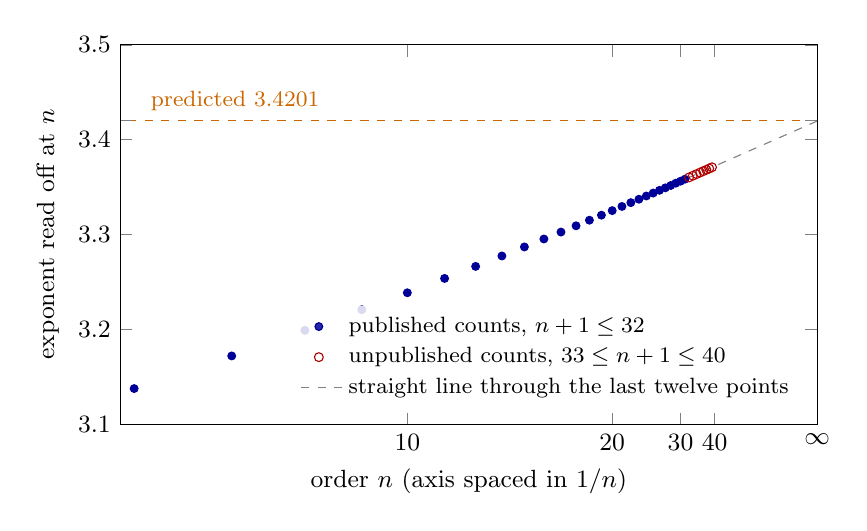
\begin{tikzpicture}
\begin{axis}[width=0.86\textwidth,height=6.4cm,xmin=0,xmax=0.17,ymin=3.1,ymax=3.5,x dir=reverse,
  xlabel={order $n$ (axis spaced in $1/n$)},ylabel={exponent read off at $n$},
  xtick={0,0.025,0.03333,0.05,0.1},xticklabels={$\infty$,$40$,$30$,$20$,$10$},
  extra y ticks={3.4201},extra y tick labels={},extra y tick style={grid=major,grid style={dashed,orange!80!black}},
  legend image post style={xscale=-1},legend cell align=left,
  legend style={font=\footnotesize,at={(0.98,0.04)},anchor=south east,draw=none,fill=white,fill opacity=0.85,text opacity=1},
  tick label style={font=\small},label style={font=\small}]
\addplot[only marks,mark=*,mark size=1.4pt,blue!60!black] coordinates {(0.16667,3.1377) (0.14286,3.1721) (0.12500,3.1991) (0.11111,3.2208) (0.10000,3.2387) (0.09091,3.2538) (0.08333,3.2665) (0.07692,3.2775) (0.07143,3.2870) (0.06667,3.2954) (0.06250,3.3027) (0.05882,3.3093) (0.05556,3.3152) (0.05263,3.3205) (0.05000,3.3253) (0.04762,3.3297) (0.04545,3.3337) (0.04348,3.3373) (0.04167,3.3407) (0.04000,3.3438) (0.03846,3.3467) (0.03704,3.3493) (0.03571,3.3518) (0.03448,3.3542) (0.03333,3.3563) (0.03226,3.3584)};
\addlegendentry{published counts, $n+1\le32$}
\addplot[only marks,mark=o,mark size=1.6pt,red!70!black] coordinates {(0.03125,3.3603) (0.03030,3.3621) (0.02941,3.3638) (0.02857,3.3654) (0.02778,3.3669) (0.02703,3.3683) (0.02632,3.3697) (0.02564,3.3710)};
\addlegendentry{unpublished counts, $33\le n+1\le40$}
\addplot[dashed,gray,domain=0:0.045] {3.4197-1.9010*x};
\addlegendentry{straight line through the last twelve points}
\node[font=\footnotesize,orange!80!black,anchor=south west] at (axis cs:0.165,3.4201) {predicted $3.4201$};
\end{axis}
\end{tikzpicture}
\caption{The exponent read off from consecutive exact counts $M_n$ and $M_{n+1}$,
$6\le n\le 39$, using the numerical estimate $\mu=12.262874$. Filled dots use published counts
($n+1\le 32$)~\cite{JG,JensenGit}. Open circles use the counts for $33\le n+1\le 40$, which were
computed privately and have not been published or independently checked. The gray line, fitted
through the last twelve points, is only a guide to the eye.}
\label{fig:readoff}
\end{figure}

This is a picture, not a measurement. Careful fits with several correction terms are consistent
with $\alpha_*$ to about three decimal places: Jensen and Guttmann estimated
$\alpha=3.4208\pm0.0006$~\cite{JG}, and a fit in this project to all $40$ counts gives
$3.4205\pm0.0004$ (Appendix~\ref{app:repo}). The second fit uses the counts for $33\le n\le40$,
which have not been checked. The data are consistent with a polynomial correction whose exponent differs from $3$, the
value for pairs of arch systems. The existence of such an asymptotic correction remains unproved.

\subsection{A meander as a walk in the quarter plane}\label{sec:quarter}

There is an appealing shortcut to $\alpha$, and it is instructive to see why it fails. Draw a
vertical line between two crossings and record two numbers: the number of arches
below the river and the number above the river that cross the line. Each crossing changes each
number by one, so a meander becomes a walk in the quarter plane that starts and ends near the
corner.

For pairs of arch systems without the one-loop requirement, the two coordinates are two
independent walks of the kind in~\eqref{eq:catalan}, and the exponent $3=3/2+3/2$ follows. More
generally, consider walks with small independent steps in the quarter plane whose two coordinates
have correlation $r$. The number of such walks that stay in the quarter plane and return to the
corner decays with the exponent $1+\pi/\arccos(-r)$~\cite{DW}; at $r=0$ this is $3$. The meander value $3.4201$ would
need $r\approx -0.27$. One could try to measure the correlation in meanders and read off the
exponent. This does not work, for two reasons.

\begin{itemize}
\item The correlation is not $-0.27$. In sampled meanders of order $512$ it is about $-0.19$
for single steps and about $-0.08$ over blocks of $8$ to $64$ steps.
\item The available measurements do not justify a Brownian approximation. Over the sampled range,
the typical size is fitted by $n^{0.52}$; finite-size data alone cannot determine the limiting scaling.
\end{itemize}

The two numbers forget how the open arches are joined to each other, and whether a crossing
closes a loop too early depends on exactly that. The walk organizes computations, but it does not
determine the exponent.

\subsection{The tape machine}\label{sec:tape}

The quarter-plane walk forgets how the open arches are joined. Paper~B~\cite{PaperB} keeps exactly
the information that matters, in a short word in two letters called the \emph{tape}.
Figure~\ref{fig:film} shows the idea before any definitions.

Draw a vertical line, the \emph{sweep line}, between two neighboring crossings and cover
everything to its right. Intuitively, this is like sliding a piece of paper from left to right along the
meander, stopping between two crossings. The sweep line meets a few pieces of road below the river, then
the river itself, then a few pieces of road above. These pieces of road are the \emph{open}
arches: they have started but not yet ended. Each object met by the sweep line gets a letter, \tape{+}
or \tape{-}, and reading the letters from bottom to top gives the tape. The letter on the river
is marked with a square in the figure and with brackets in the text; it is the \emph{head}. As
the paper slides past one more crossing, the tape changes only next to the head.

\begin{figure}[ht]
\centering
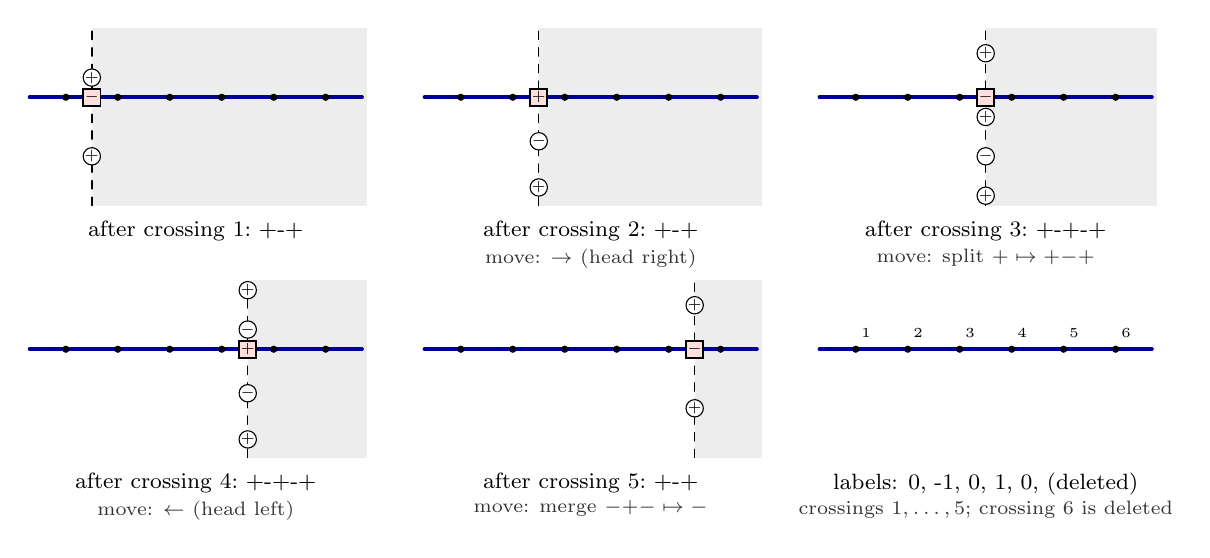
\begin{tikzpicture}[x=0.66cm,y=0.5cm,line cap=round]
\begin{scope}[shift={(0.00,0.00)}]
  \fill[black!7] (1.50,-2.75) rectangle (6.8,1.75);
  \draw[blue!60!black,line width=1.3pt] (0.3,0)--(6.7,0);
  \begin{scope}[black!25,line width=0.6pt]\meanderroad\end{scope}
  \begin{scope}\clip (0.3,-2.75) rectangle (1.50,1.75);\begin{scope}[line width=1pt]\meanderroad\end{scope}\end{scope}
  \draw[dashed,line width=0.5pt] (1.50,-2.75)--(1.50,1.75);
  \foreach \k in {1,...,6} {\fill (\k,0) circle[radius=1.3pt];}
  \draw[fill=white,line width=0.4pt] (1.50,-1.500) circle[radius=0.11cm]; \node[font=\tiny,inner sep=0pt] at (1.50,-1.500) {$+$};
  \draw[fill=red!13,line width=0.7pt] (1.50,0) ++(-0.11cm,-0.11cm) rectangle ++(0.22cm,0.22cm); \node[font=\tiny,inner sep=0pt] at (1.50,0) {$-$};
  \draw[fill=white,line width=0.4pt] (1.50,0.500) circle[radius=0.11cm]; \node[font=\tiny,inner sep=0pt] at (1.50,0.500) {$+$};
  \node[font=\footnotesize,anchor=north] at (3.5,-2.9) {after crossing 1:\ \tape{+}\hd{-}\tape{+}};
\end{scope}
\begin{scope}[shift={(7.60,0.00)}]
  \fill[black!7] (2.50,-2.75) rectangle (6.8,1.75);
  \draw[blue!60!black,line width=1.3pt] (0.3,0)--(6.7,0);
  \begin{scope}[black!25,line width=0.6pt]\meanderroad\end{scope}
  \begin{scope}\clip (0.3,-2.75) rectangle (2.50,1.75);\begin{scope}[line width=1pt]\meanderroad\end{scope}\end{scope}
  \draw[dashed,line width=0.5pt] (2.50,-2.75)--(2.50,1.75);
  \foreach \k in {1,...,6} {\fill (\k,0) circle[radius=1.3pt];}
  \draw[fill=white,line width=0.4pt] (2.50,-2.291) circle[radius=0.11cm]; \node[font=\tiny,inner sep=0pt] at (2.50,-2.291) {$+$};
  \draw[fill=white,line width=0.4pt] (2.50,-1.118) circle[radius=0.11cm]; \node[font=\tiny,inner sep=0pt] at (2.50,-1.118) {$-$};
  \draw[fill=red!13,line width=0.7pt] (2.50,0) ++(-0.11cm,-0.11cm) rectangle ++(0.22cm,0.22cm); \node[font=\tiny,inner sep=0pt] at (2.50,0) {$+$};
  \node[font=\footnotesize,anchor=north] at (3.5,-2.9) {after crossing 2:\ \tape{+}\tape{-}\hd{+}};
  \node[font=\scriptsize,anchor=north,gray!40!black] at (3.5,-3.6) {move: $\to$ (head right)};
\end{scope}
\begin{scope}[shift={(15.20,0.00)}]
  \fill[black!7] (3.50,-2.75) rectangle (6.8,1.75);
  \draw[blue!60!black,line width=1.3pt] (0.3,0)--(6.7,0);
  \begin{scope}[black!25,line width=0.6pt]\meanderroad\end{scope}
  \begin{scope}\clip (0.3,-2.75) rectangle (3.50,1.75);\begin{scope}[line width=1pt]\meanderroad\end{scope}\end{scope}
  \draw[dashed,line width=0.5pt] (3.50,-2.75)--(3.50,1.75);
  \foreach \k in {1,...,6} {\fill (\k,0) circle[radius=1.3pt];}
  \draw[fill=white,line width=0.4pt] (3.50,-2.500) circle[radius=0.11cm]; \node[font=\tiny,inner sep=0pt] at (3.50,-2.500) {$+$};
  \draw[fill=white,line width=0.4pt] (3.50,-1.500) circle[radius=0.11cm]; \node[font=\tiny,inner sep=0pt] at (3.50,-1.500) {$-$};
  \draw[fill=white,line width=0.4pt] (3.50,-0.500) circle[radius=0.11cm]; \node[font=\tiny,inner sep=0pt] at (3.50,-0.500) {$+$};
  \draw[fill=red!13,line width=0.7pt] (3.50,0) ++(-0.11cm,-0.11cm) rectangle ++(0.22cm,0.22cm); \node[font=\tiny,inner sep=0pt] at (3.50,0) {$-$};
  \draw[fill=white,line width=0.4pt] (3.50,1.118) circle[radius=0.11cm]; \node[font=\tiny,inner sep=0pt] at (3.50,1.118) {$+$};
  \node[font=\footnotesize,anchor=north] at (3.5,-2.9) {after crossing 3:\ \tape{+}\tape{-}\tape{+}\hd{-}\tape{+}};
  \node[font=\scriptsize,anchor=north,gray!40!black] at (3.5,-3.6) {move: split $\tape{+}\mapsto\tape{+}\hd{-}\tape{+}$};
\end{scope}
\begin{scope}[shift={(0.00,-6.40)}]
  \fill[black!7] (4.50,-2.75) rectangle (6.8,1.75);
  \draw[blue!60!black,line width=1.3pt] (0.3,0)--(6.7,0);
  \begin{scope}[black!25,line width=0.6pt]\meanderroad\end{scope}
  \begin{scope}\clip (0.3,-2.75) rectangle (4.50,1.75);\begin{scope}[line width=1pt]\meanderroad\end{scope}\end{scope}
  \draw[dashed,line width=0.5pt] (4.50,-2.75)--(4.50,1.75);
  \foreach \k in {1,...,6} {\fill (\k,0) circle[radius=1.3pt];}
  \draw[fill=white,line width=0.4pt] (4.50,-2.291) circle[radius=0.11cm]; \node[font=\tiny,inner sep=0pt] at (4.50,-2.291) {$+$};
  \draw[fill=white,line width=0.4pt] (4.50,-1.118) circle[radius=0.11cm]; \node[font=\tiny,inner sep=0pt] at (4.50,-1.118) {$-$};
  \draw[fill=red!13,line width=0.7pt] (4.50,0) ++(-0.11cm,-0.11cm) rectangle ++(0.22cm,0.22cm); \node[font=\tiny,inner sep=0pt] at (4.50,0) {$+$};
  \draw[fill=white,line width=0.4pt] (4.50,0.500) circle[radius=0.11cm]; \node[font=\tiny,inner sep=0pt] at (4.50,0.500) {$-$};
  \draw[fill=white,line width=0.4pt] (4.50,1.500) circle[radius=0.11cm]; \node[font=\tiny,inner sep=0pt] at (4.50,1.500) {$+$};
  \node[font=\footnotesize,anchor=north] at (3.5,-2.9) {after crossing 4:\ \tape{+}\tape{-}\hd{+}\tape{-}\tape{+}};
  \node[font=\scriptsize,anchor=north,gray!40!black] at (3.5,-3.6) {move: $\leftarrow$ (head left)};
\end{scope}
\begin{scope}[shift={(7.60,-6.40)}]
  \fill[black!7] (5.50,-2.75) rectangle (6.8,1.75);
  \draw[blue!60!black,line width=1.3pt] (0.3,0)--(6.7,0);
  \begin{scope}[black!25,line width=0.6pt]\meanderroad\end{scope}
  \begin{scope}\clip (0.3,-2.75) rectangle (5.50,1.75);\begin{scope}[line width=1pt]\meanderroad\end{scope}\end{scope}
  \draw[dashed,line width=0.5pt] (5.50,-2.75)--(5.50,1.75);
  \foreach \k in {1,...,6} {\fill (\k,0) circle[radius=1.3pt];}
  \draw[fill=white,line width=0.4pt] (5.50,-1.500) circle[radius=0.11cm]; \node[font=\tiny,inner sep=0pt] at (5.50,-1.500) {$+$};
  \draw[fill=red!13,line width=0.7pt] (5.50,0) ++(-0.11cm,-0.11cm) rectangle ++(0.22cm,0.22cm); \node[font=\tiny,inner sep=0pt] at (5.50,0) {$-$};
  \draw[fill=white,line width=0.4pt] (5.50,1.118) circle[radius=0.11cm]; \node[font=\tiny,inner sep=0pt] at (5.50,1.118) {$+$};
  \node[font=\footnotesize,anchor=north] at (3.5,-2.9) {after crossing 5:\ \tape{+}\hd{-}\tape{+}};
  \node[font=\scriptsize,anchor=north,gray!40!black] at (3.5,-3.6) {move: merge $\tape{-}\hd{+}\tape{-}\mapsto\hd{-}$};
\end{scope}
\begin{scope}[shift={(15.20,-6.40)}]
  \draw[blue!60!black,line width=1.3pt] (0.3,0)--(6.7,0);
  \begin{scope}[line width=1pt]\meanderroad\end{scope}
  \foreach \k in {1,...,6} {\fill (\k,0) circle[radius=1.3pt]; \node[fill=white,inner sep=0.5pt,font=\tiny] at (\k+0.2,0.4) {\k};}
  \node[font=\footnotesize,anchor=north] at (3.5,-2.9) {labels: 0,\ -1,\ 0,\ 1,\ 0,\ (deleted)};
  \node[font=\scriptsize,anchor=north,gray!40!black] at (3.5,-3.6) {crossings $1,\dots,5$; crossing $6$ is deleted};
\end{scope}
\end{tikzpicture}

\caption{The tape machine on the meander of Figure~\ref{fig:meander}. In each panel the part of
the meander right of the dashed sweep line is covered (gray). The sweep line meets the open arches below the
river, the river (square: the head), and the open arches above; their letters, read from bottom
to top, form the tape. Passing one crossing changes the tape by one move, named under each panel.
The last panel shows the labels from which the letters are computed.}
\label{fig:film}
\end{figure}

The letters come from a numbering of the crossings. Delete the last crossing; the road, which
was a closed loop, becomes a single path through the other crossings. Give the first crossing the
\emph{label} $0$ and walk along the path: the label drops by one along an arch above the river,
read from left to right, and rises by one along an arch below the river. Intuitively, the label
counts the half turns of the road, with turns above and below the river counted with opposite
signs. A planar argument shows that neighboring crossings along the river have labels that differ
by exactly one. Now give each gap between two objects on the sweep line a number: $-1$ for the gap below
everything, $0$ for the gap above everything, the label of its left end for the gap just above
an open arch below the river, and that label minus one for the gap just below an open arch above
the river. Neighboring gap numbers differ by exactly one, and the letter of each object says
whether the number goes up (\tape{+}) or down (\tape{-}) across it.

\begin{theorem}[the tape machine~\cite{PaperB}]\label{thm:tape}
A \emph{tape} is a word in \tape{+} and \tape{-} with one marked letter, the head, written in
brackets. A \emph{move} does one of the following: move the head one letter left or right; replace
a head \tape{+} by \tape{+}\hd{-}\tape{+}; replace a head \tape{-} by \tape{+}\hd{-}\tape{-} or by
\tape{-}\hd{-}\tape{+}; or replace a head \tape{+} together with its two neighbors by a single
head letter, which is \tape{-} if both neighbors are \tape{-} and \tape{+} otherwise. This last
move is not allowed when both neighbors are \tape{+}, that is, at \tape{+}\hd{+}\tape{+}. Then
the meanders of order $n$ are in one-to-one correspondence with the sequences of $2n-2$ moves that
start at the tape \tape{+}\hd{-}\tape{+} and end at it.
\end{theorem}

\begin{figure}[t]
\centering
\begin{tikzpicture}[>=stealth]
  \tp{(0,0)}{+,-,+,-,+}{4}
  \tp{(2.6,1.35)}{+,-,+,-,+}{3} \draw[->,line width=0.5pt] (1.95,0)--(2.5,1.35); \node[font=\scriptsize,anchor=west] at (5.05,1.35) {head left};
  \tp{(2.6,0.45)}{+,-,+,-,+}{5} \draw[->,line width=0.5pt] (1.95,0)--(2.5,0.45); \node[font=\scriptsize,anchor=west] at (5.05,0.45) {head right};
  \tp{(2.6,-0.45)}{+,-,+,+,-,-,+}{5} \draw[->,line width=0.5pt] (1.95,0)--(2.5,-0.45); \node[font=\scriptsize,anchor=west] at (5.05,-0.45) {split};
  \tp{(2.6,-1.35)}{+,-,+,-,-,+,+}{5} \draw[->,line width=0.5pt] (1.95,0)--(2.5,-1.35); \node[font=\scriptsize,anchor=west] at (5.05,-1.35) {split};
  \node[font=\small,anchor=east] at (-0.1,0) {(a)};
  \begin{scope}[xshift=7.9cm]
  \tp{(0,0)}{+,-,+,-,+}{3}
  \tp{(2.6,1.35)}{+,-,+,-,+}{2} \draw[->,line width=0.5pt] (1.95,0)--(2.5,1.35); \node[font=\scriptsize,anchor=west] at (5.05,1.35) {head left};
  \tp{(2.6,0.45)}{+,-,+,-,+}{4} \draw[->,line width=0.5pt] (1.95,0)--(2.5,0.45); \node[font=\scriptsize,anchor=west] at (5.05,0.45) {head right};
  \tp{(2.6,-0.45)}{+,-,+,-,+,-,+}{4} \draw[->,line width=0.5pt] (1.95,0)--(2.5,-0.45); \node[font=\scriptsize,anchor=west] at (5.05,-0.45) {split};
  \tp{(2.6,-1.35)}{+,-,+}{2} \draw[->,line width=0.5pt] (1.95,0)--(2.5,-1.35); \node[font=\scriptsize,anchor=west] at (5.05,-1.35) {merge};
  \node[font=\small,anchor=east] at (-0.1,0) {(b)};
  \end{scope}
\end{tikzpicture}
\caption{All moves from two tapes of Figure~\ref{fig:film}; the shaded box is the head.
(a) From \tape{+-+}\hd{-}\tape{+} (after crossing $3$), with the head on a \tape{-}: two head
moves and two splits. (b) From \tape{+-}\hd{+}\tape{-+} (after crossing $4$), with the head on a
\tape{+}: two head moves, one split, and the merge, which returns to the starting tape.}
\label{fig:moves}
\end{figure}

The moves match the four kinds of crossing. A crossing opens or closes one arch above and one
below the river. Opening on one side and closing on the other moves the head; opening on both
sides replaces one letter by three (a \emph{split}); closing on both sides replaces three letters
by one (a \emph{merge}). Figure~\ref{fig:moves} shows every move available at two tapes. The first
crossing creates the starting tape and the last closes the final two arches, so a meander of order
$n$, with $2n$ crossings, gives $2n-2$ moves. In Figure~\ref{fig:film} the four moves are head
right, split, head left and merge.

Each move reads and changes only the head and its two neighbors, so the global one-loop condition
has become a set of local rules. The merge at \tape{+}\hd{+}\tape{+} is excluded because no
consistent labels could follow it: after it, the open arches would force the next label to go
down and up at once. Conversely, a planar argument shows that labels obeying the local rules always
come from a single closed road. For $n=2$ there are exactly two sequences,
\[ \tape{+}\hd{-}\tape{+} \to \hd{+}\tape{-+} \to \tape{+}\hd{-}\tape{+}
\qquad\text{and}\qquad
\tape{+}\hd{-}\tape{+} \to \tape{+-}\hd{+} \to \tape{+}\hd{-}\tape{+},\]
matching the two meanders of order $2$. Enumerating the sequences by computer reproduces
$1, 2, 8, 42, 262, 1828$ for $n\le 6$.

In this picture $M_n$ literally counts walks that come back to their start, as in the first
subsection: walks on the set of tapes. The growth rate $\mu$ is the growth rate of the number of
such walks, and $\alpha$ is the conjectured power-law correction after the factor $\mu^n$ is removed. But the set
of tapes is infinite, and the walk is not close to a Brownian motion, which is why the reasoning
of the first subsection does not produce $\alpha$ directly.

The tape machine is behind the best current bounds on $\mu$, proved in Paper~B,
\[ 12.2191\;\le\;\mu\;\le\;12.2970 .\]
The upper bound uses two positive weights, one looking forward along the moves and one looking
backward. Their paired inequalities control a symmetric operator on every finite set of tapes.
This bounds the number of closed move sequences, and hence the exponential growth of $M_n$,
by $12.2970$ per order.
The lower bound comes from a random rule for choosing moves that looks only at the letters near
the head, keeps the tape statistically the same over time, and on average neither lengthens the
tape nor moves the head to one side. Its \emph{entropy}, the average over the choices it makes
of the logarithm of one over the probability of the choice, is at least $\log 12.2191$ per two
moves. Intuitively, such a rule makes in effect about $12.2191$ equally likely choices per two
moves, so it produces about $12.2191^n$ different sequences of $2n$ moves. These sequences can be
closed into meanders at small cost, which gives $\mu\ge12.2191$. Both certificates were checked in exact arithmetic, and each was checked again by a
separately written program; for the lower bound, part of this second check covers a sample of
the equations rather than all of them. Paper~B explains both certificates; it supersedes an
earlier account of the weight method in this project~\cite{BoundsPaper}. The best bounds
published in a journal are $11.380\le\mu\le12.901$~\cite{AP}, and recent certified computations
and preprints give $11.6080\le\mu\le12.6319$~\cite{Fox} and $\mu\le12.806$~\cite{CDDV}.

\subsection{Meanders with bounded labels}\label{sec:band}

Restricting the labels to a fixed range makes the machine much simpler, and then the exponent
can be computed exactly. For the meanders whose labels all lie between $-1$ and $2$ the following
holds; the proof is in Paper~C~\cite{PaperC}.

\begin{theorem}[meanders with labels in $\{-1,0,1,2\}$]\label{thm:band}
Let $m_0=0.9175\ldots$ be the positive root of $4x^4=2x+1$. The number of meanders of order $n$
with all labels in $\{-1,0,1,2\}$ grows like $\Lambda^n$, where
$\Lambda=(1+2m_0)(1+m_0)^2=10.4245\ldots$ is the larger real root of
$16x^4-112x^3-520x^2-536x+25$. More precisely, the number is $\Lambda^n n^{-\alpha_{\mathrm b}+o(1)}$, where
\[ \alpha_{\mathrm b} \;=\; 1+\frac{\pi}{\arccos\!\big((1+2m_0)/(3+4m_0)\big)} \;=\; 3.7758\ldots \]
\end{theorem}

The exponent has the same form as the quarter-plane return exponent above: one plus $\pi$
divided by an angle. With the labels bounded, the machine has only finitely many control states,
and the two coordinates of Section~\ref{sec:quarter}, the numbers of open arches below and above
the river, behave at large scales like a planar Brownian motion with correlated coordinates. A
linear change of coordinates turns it into a standard Brownian motion and turns the quarter plane
into a wedge with opening angle $\arccos\big((1+2m_0)/(3+4m_0)\big)$, and this angle sets the
exponent. Like $\alpha_*$, the value $\alpha_{\mathrm b}$ is irrational, but for a different
reason: it comes from an angle, not from the root of a quadratic equation. For all meanders the
labels are unbounded, and no reduction of this kind is known.
